\section{Schematics}

\subsection{Page 1: TSMPPT wiring}

\begin{figure}
	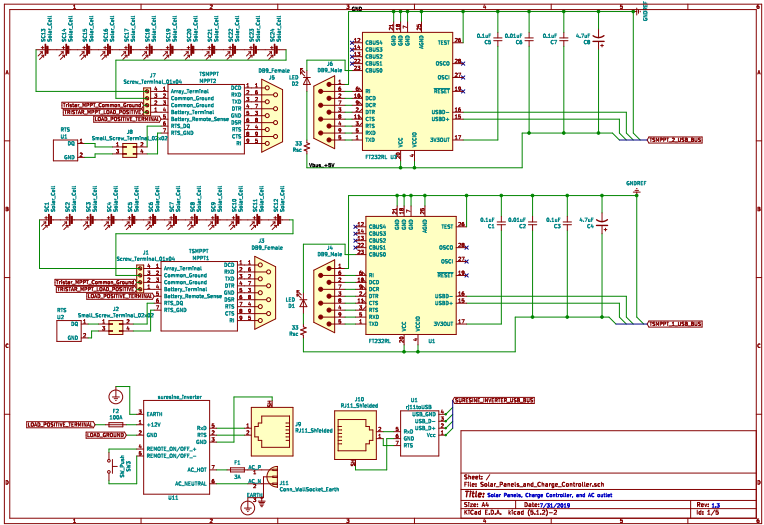
\includegraphics{./graphics/schematic/sch_page_1.png}
\end{figure}
This page contains the solar panel arrays, the Tristar MPPT boxes, the RTS boxes, the DC-AC converter, and the wall socket.
All solar panel strings are wired in series.
\newline
Wire Gauge: 
2.5mm2 / 14 AWG Minimum
35mm2 / 2 AWG Maximum 

Each solar panel string contains 12 solar panels. The solar panel voltages add up to $8V*12 = 96V$ on average.
The Tristar MPPT box has large screw terminals to connect the solar panel array and the batteries to charge. The connection for the battery remote sense only has a single small screw terminal, and the RTS has a double small screw terminal, for these connections: RTS\_DQ, and RTS\_GND.

The Tristar MPPT box also has a female DB9 output for RS-232 communication.

Each solar panel string is connected to the Tristar MPPT box like this: 
Positive end of solar panel string connects to the Array Positive Terminal, and the negative end of solar panel string connects to the first common ground terminal.
\newline
Wire Gauge: 
2.5mm2 / 14 AWG Minimum
35mm2 / 2 AWG Maximum 

The battery array connects to the Tristar MPPT box like this:
There are special terminals on page 2 that are reserved to connect to the Tristar MPPT box. They are called Tristar\_MPPT\_Positive and Tristar\_MPPT\_Common\_Ground. Tristar\_MPPT\_Positive connects to the battery terminal, and Tristar\_MPPT\_Common\_Ground connects to the second common ground terminal.
\newline
Wire Gauge: 
2.5mm2 / 14 AWG Minimum
35mm2 / 2 AWG Maximum 

The Raspberry Pi connects to the Tristar MPPT box like this:

There exists a RS-232 to USB converter cable. The RS-232 to USB cable has a Male DB9 input, and a Male USB type B output. I put its schematics in my schematic. It uses a FT232RL chip. Its inputs are the standard inputs from a RS-232 pinout (RI, DCD,DCR,DTR,CTS,RTS,RXD, TXD,GND). The FT232RL chip gets its power from the USB power wire (+5V). Its outputs are the 4 wires of a USB 2.0 interface. It is terminated by 2 global busses: TSMPPT\_1\_USB\_BUS, and TSMPPT\_2\_USB\_BUS.
\newline
Any RS-232 to USB cable will do.

The suresine inverter is a Morningstar product. It takes 12V, and outputs a pure 110V 50Hz sine wave. See datasheet. There is a Remote on/off feature, but we will not be taking advantage of that. Instead, we will be wiring a push button across it, and having it always on.
The suresine inverter requires a 3A fuse on the AC\_P line of the wall socket, and a 100A fuse on the LOAD\_POSITIVE\_TERMINAL input. That way, nobody dies from overcurrent. 

The suresine inverter has a Meterbus output, in the form of an RJ-11 output. There are 3 wires for this interface: RxD, RTS, and GND. It uses a RJ11 phone cable to communicate to a Meterbus converter to USB. See components document for information about it. It’s powered by the USB power line (+5V). We can acquire a Morningstar Meterbus converter from multiple sources, but Morningstar itself is the best source. The final output of the Morningstar Meterbus converter is a 4-wire USB bus, terminated by a global bus header, named SURESINE\_INVERTER\_USB\_BUS.
\newline
Any RJ-11 cable will do.

The suresine inverter also requires a connection to the earth. We are using a grounded wall socket for safety, per GFCI standards. There is a connection to earth on the suresine inverter, and a connection to earth on the wall socket. 
\newline
Wire Gauge: 
2.5mm2 / 14 AWG Minimum
35mm2 / 2 AWG Maximum 

\subsection{Page 2: Batteries}

\begin{figure}
	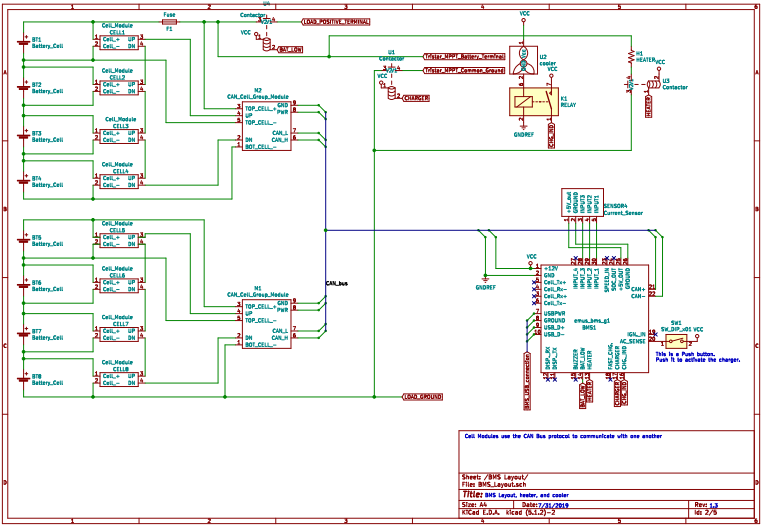
\includegraphics{./graphics/schematic/sch_page_2.png}
\end{figure}

This page contains the batteries and the battery management system.

Every Battery Cell is a 3.2V lithium ion battery from CALB. See the datasheet. It can output 520Ah of power. We want a 12V battery pack, so we must have batteries in groups of 4. The batteries are wired in series, so we get 12.8V. We should have 8 batteries in total, so that means 2 groups.
\newline
Wire Gauge: 
2.5mm2 / 14 AWG Minimum
35mm2 / 2 AWG Maximum 

\subsubsection{Cell intra-communication}
Each battery has its own cell module. Each cell module has 4 inputs: Cell + (the positive side of the battery), Cell – (the negative side of the battery), UP and DN (for CAN bus communication. The battery is connected to Cell + on the positive side, and Cell – on the negative side. 

If the battery is the first one in the group, then the UP connection goes to the UP connection of the CAN Cell group module. If not, the UP connection goes to the DN connection of the previous Cell module. If the battery is the last one in the group, the DN connection goes to the DN connection of the CAN Cell Group module. Otherwise, it connects to the UP connection of the next cell module.

Each CAN Cell Group Module handles all batteries within its specified group. Its connections go like this:

\begin{itemize}
	\item TOP CELL +: Goes to the positive side of the first battery.
	\item TOP CELL -: Goes to the negative side of the first battery.
	\item UP: Goes to the UP connection of the first cell module.
	\item DN: Goes to the DN connection of the last cell module. 
	\item BOT CELL -: Goes to the negative side of the last battery.
	\item GND: Goes to the GROUND of the master EMUS BMS unit.
	\item PWR: Goes to Vcc (+12V) of this page (also +12V of master EMUS BMS unit.
	\item CAN\_L: Goes to CAN – of the master EMUS BMS unit.
	\item CAN\_H: Goes to CAN + of the master EMUS BMS unit.
\end{itemize}
PLC reading:
The EMUS BMS unit has its own 4-wire USB interface. All of those connections combine into a USB bus, terminated in a header called BMS\_USB\_CONNECTION.
Distributing Power:
The load is connected to LOAD\_POSITIVE and LOAD\_GROUND. The BMS control unit will control how much current is dissipated based on the battery health and the voltage demanded (12V).
Heating and Cooling:
The HEATER and CHG\_IND pins are connected to relays that actuate a heater or a cooler respectively. The internal PLC of the BMS system controls when they are actuated. The BMS system is automatically calibrated towards Lithium-Ion batteries.
The BAT\_LOW pin is connected to a contactor. It controls when power is going to be distributed at all or not.
There is a current sensor on the schematic. It’s connected to the BMS system via 5 pins: INPUT1, INPUT2, INPUT3, +5V\_out, and GND. It’s a hall effect sensor, so it’s shaped like a ring. You must put the current sensor through the wire going to the load. The wire goes on the inside of the current sensor. 
Disconnected Terminals on the BMS header:
DISP\_RX and DISP\_TX: these are used for LCD displays sold by Emus. I don’t think it’s necessary.
BUZZER: This is used to activate a buzzer. We don’t want one.
FAST\_CHG. : This is used for CAN-based chargers. We don’t have one. We have an analog chager.
IGN\_IN: this is used for electric vehicles. We’re not implementing this system in an electrical vehicle, so we won’t use it.
INPUT\_4, SPEED\_IN, SOC\_OUT: These are extra pins that EMUS put in for future use. We don’t need any of those.
CELL\_Tx+, Cell\_Rx-, Cell\_Rx-+, Cell\_Tx-: These aren’t used for anything important.

Miscellaneous:
The AC\_SENSE pin is connected to a push-button. It is mandatory that we have this connected. We should have a push button tomorrow.

\subsection{Page 3: Raspberry Pi}
\begin{figure}
	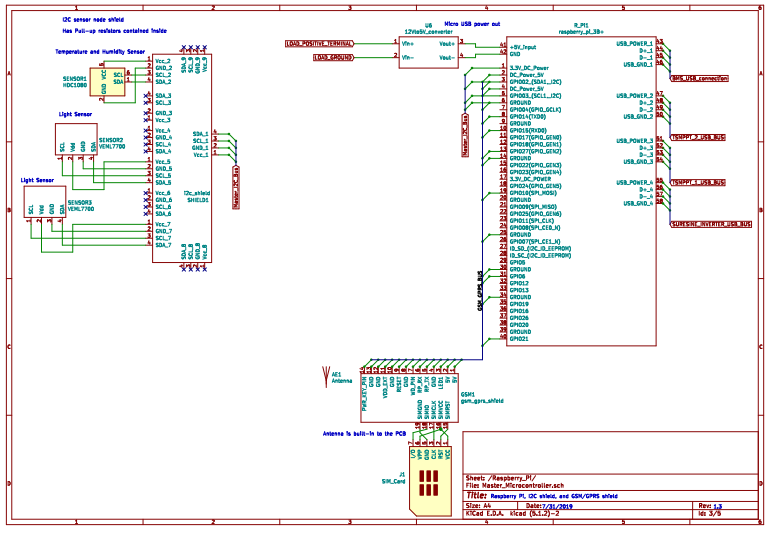
\includegraphics{./graphics/schematic/sch_page_3.png}
\end{figure}
This page contains the Raspberry Pi, the I2C shield, the GSM/GPRS shield, and the sensors. Also has a box representing the 12V converter. That’s explained on page 4 of the schematic.

\subsubsection{Raspberry Pi}
This is the main processing unit. It contains all of my code. It needs 5V to operate. Tolerances: 4.5V to 5.5V. I need a stable power supply. That’s on another page. It has 4 USB ports on it. Each one is being used for a different purpose. There is a Master I2C bus going to the I2C shield. There won’t be wires. It will be with a 22-pin header. It will have a lot of “no-connect” pins on it, but it will fit perfectly on top of the Raspberry Pi.

\subsubsection{I2C shield}

This is an expansion of an I2C shield. I absolutely need it, since the Raspberry Pi only has 1 I2C port on it. We can expand it by having an I2C shield. We can put it on top.

\subsubsection{GSM/GPRS shield}
This is a shield that allows one to use a Ting 2G connection to the internet. I will be utilizing it to send JSON files over the internet to a server via TCP protocols. In both Python and C++, there are libraries used to deal with the HTTP/TCP interface that the internet requires. The chip used on this GSM/GPRS shield uses AT commands. Luckily, in both Python and C++, there are AT command libraries.
There is an internal SIM card slot. I marked it on the schematic. It’s a 6-pin scheme. It’s meant to read a 16-bit number on your SIM card: your ID number. It’s very important to have this ID number embedded in your GSM shield so that the cell phone tower that receives it knows that you are authorized to use its cell towers. (coincidentally, this is why 911 works everywhere. It’s one of the few numbers that is required by law to be let through regardless of whether you have paid for an authentication number.)

\subsubsection{Physical connection}
GSM/GPRS shield has a 22-pin header already on the board. It’s made by SixFab. It will connect directly to the Raspberry Pi. It can also act as a go-between between the Raspberry Pi and the I2C shield. It will be the meat between a Raspberry Pi and I2C shield sandwich. It just requires a long header.

As far as antennas are concerned, you can either use the built-in PCB antenna, or you can connect your own antenna. It has a standardized connector for Microcontroller-style antennas.
\subsubsection{Sensors}
All our sensors are ordered as breakout boards (the VEML7700 and the HDC1080). I will have to design something that lets you connect to the I2C shield without too much hassle.

\subsection{Page 4: DC-DC Converter}
\begin{figure}
	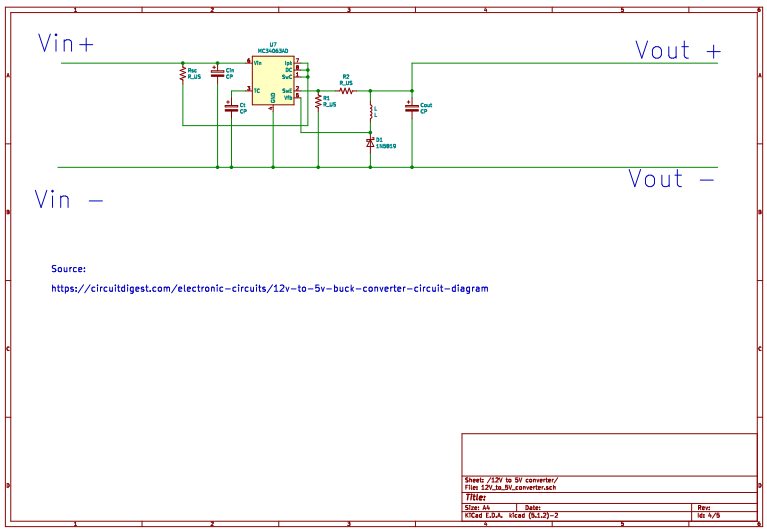
\includegraphics{./graphics/schematic/sch_page_4.png}
\end{figure}
This page contains the internal schematics of a 12V to 5V DC-DC converter, and the source from which I got it from.
The one I propose uses the MC34063AD microchip. I don’t know what the values are for the resistors, capacitors and the inductors are, but It’s probably in the source.
Vin+ is +12V.
Vin- is GND.
Vout+ is +5V.
Vout- is GND.
Vout must also be in the form of a Micro-USB type A connector. That is what the raspberry pi uses.
\subsection{Page 5: Student Sensor Reader}
\begin{figure}
	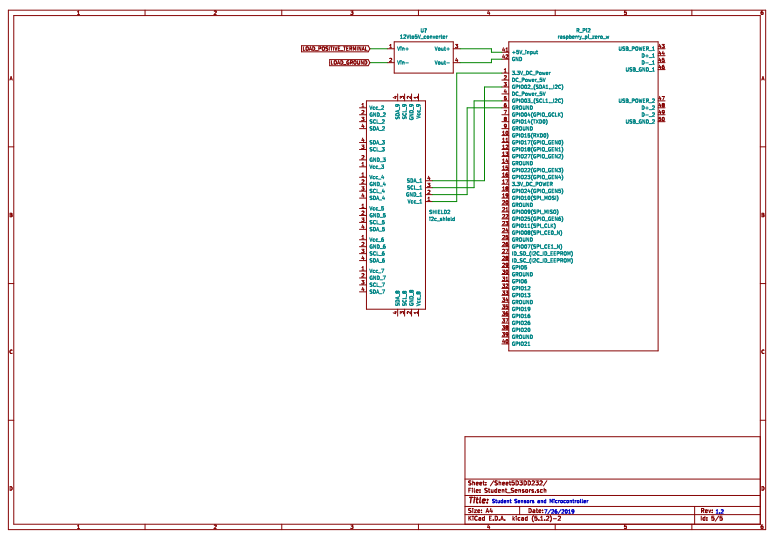
\includegraphics{./graphics/schematic/sch_page_5.png}
\end{figure}
This page contains the slave microcontroller (a Raspberry Pi zero w), another 12V to 5V converter, and another I2C shield.
It also has a 22-pin header, so it can connect to the I2C shield just as easily as any other. 

